% This presentation introduces a decision-centric framework for inventory planning that explicitly models and propagates uncertainty throughout the forecasting and optimization pipeline. We begin by motivating the need for probabilistic forecasts through the classical newsvendor problem, showing that optimal inventory decisions depend on the entire demand distribution rather than point estimates alone. We then discuss several approaches to probabilistic forecasting, including Generalized Linear Models (GLMs), Generalized Additive Models for Location, Scale, and Shape (GAMLSS), and quantile regression. Next, we show how demand uncertainty can be propagated over lead times and review periods by computing the distribution of cumulative demand using convolution and mixture distributions. Finally, we formulate inventory planning as a stochastic optimization problem under working capital constraints. The central theme of this talk is that forecasting is not an end in itself; rather, probabilistic forecasts should be viewed as inputs to downstream decision-making systems that optimize inventory under uncertainty.

\documentclass[11pt]{beamer}
\usetheme{Madrid}
\usecolortheme{whale}

\usepackage[utf8]{inputenc}
\usepackage[english]{babel}
\usepackage{amsfonts, amsmath, amssymb} % For math formatting
\usepackage{graphicx} % For importing images
\usepackage{alphalph}

\usepackage[
backend=biber,
style=authoryear,
]{biblatex}
\bibliography{mybib.bib}

\addtobeamertemplate{footnote}{}{\vspace{2ex}}
% \renewcommand{\thefootnote}{\alph{footnote}}
\renewcommand{\thefootnote}{[\arabic{footnote}]}

\title[Probablistic Forecasting]{Decision-Centric Probabilistic Forecasting for Inventory Optimization}
\author{Shobhit Bhatnagar}
\institute{Flipkart}
\date{\today}

\AtBeginSection[]
{
    \begin{frame}
        \frametitle{Table of Contents}
        \tableofcontents[currentsection]
    \end{frame}
}

\begin{document}
\begin{frame}
	\titlepage
\end{frame}

\begin{frame}{Outline}
	\tableofcontents
\end{frame}

\section{Why Probabilistic Forecasts?}
\begin{frame}{Point Forecasts}
\begin{footnotesize}
Point forecasts predict expected demand: $\hat{D}_{i, \tau} \approx \mathbb{E}[D_{i, \tau} | x_{i, t}]$, where:

\begin{itemize}
\item $i$ = SKU / product
\item $\tau$ = future time period being forecasted
\item $t$ = decision time / forecast origin
\item $D_{i, \tau}$ = random demand for SKU $i$ at time $\tau$
\item $x_{i, t}$ = feature vector available at time $t$ for forecasting demand in period $\tau$. Example:
\begin{align*}
x_{i, t} &= \begin{bmatrix} \text{day of week}_\tau \\ \text{holiday flag}_\tau \\ \text{price}_{i, \tau} \\ \text{promotion}_{i,\tau} \\ \text{demand lags up to $t$} \\ \text{rolling demand features up to $t$} \\ \text{SKU / category / store attributes} \\ \vdots \end{bmatrix}
\end{align*}
\end{itemize}
But inventory decisions depend on \textbf{risk}, not only expected demand.
\end{footnotesize}
\end{frame}

\begin{frame}[allowframebreaks]{The Newsvendor Problem}
\begin{small}
\begin{itemize}
\item The Newsvendor Problem is a mathematical model used to determine the optimal inventory level for perishable or single-period goods.
\item It balances the cost of overstocking (unsold items) against the cost of understocking (lost profit from unmet demand) to minimize expected total cost.
\item The cost of over-forecasting and under-forecasting is asymmetric:
\begin{align*}
C(q, D) &= h (q - D)^+ + b (D - q)^+
\end{align*}
where $h$ is overage / holding / spoilage cost and $b$ is underage / lost-sales / service cost.
\item The optimal inventory is a quantile, not the mean:
\begin{align*}
q^* &= F^{-1}\left(\frac{b}{b+h}\right)
\end{align*}
where $F$ is cumulative distribution function (cdf) of the demand. 
\end{itemize}
\end{small}

\framebreak
\begin{footnotesize}
\begin{itemize}
\item For high service levels (95\%-99\%), the right tail of the demand distribution is crucial for determining the optimal inventory level.
\item Two SKUs can have the same mean but very different safety stock requirements:
\begin{align*}
\mathbb{E}[D_1] = \mathbb{E}[D_2], \quad F_1^{-1}(0.95) \neq F_2^{-1}(0.95)
\end{align*}
\end{itemize}
\end{footnotesize}

\begin{figure}
\centering
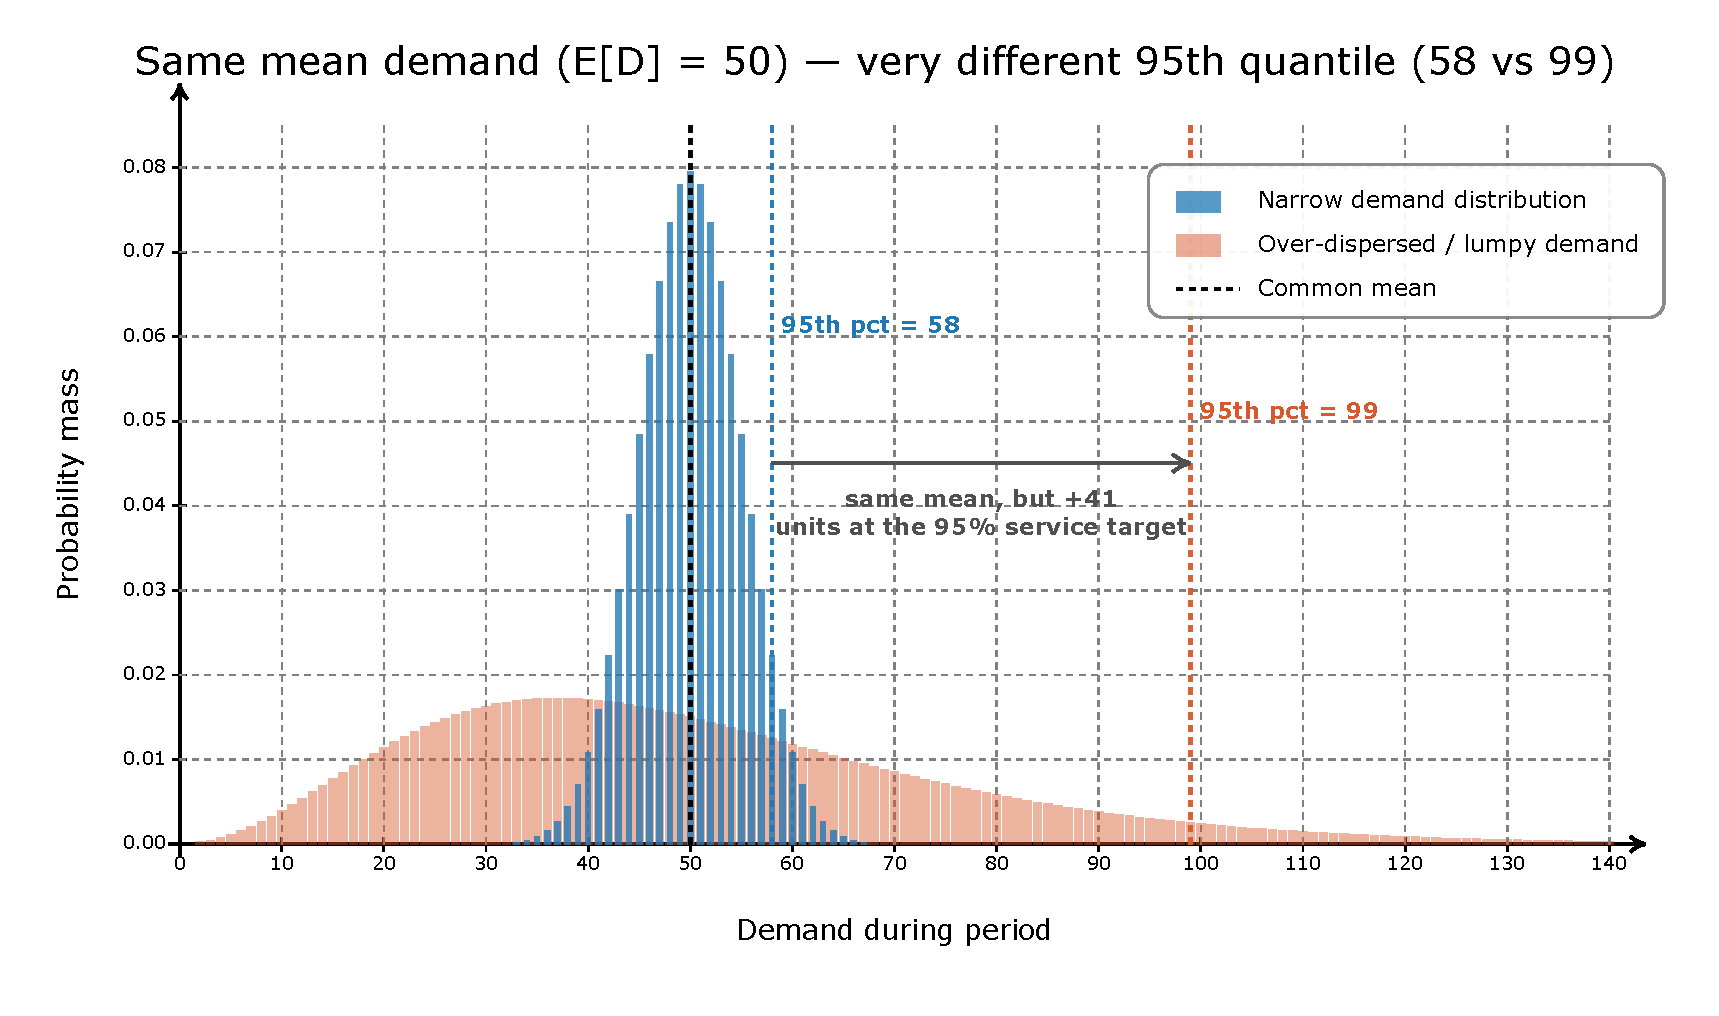
\includegraphics[width=235pt]{figures/demand_same_mean_diff_quantile.pdf}
\end{figure}

\end{frame}

\section{Techniques for Probablistic Forecasting}
\begin{frame}{Generalized Linear Models}
\begin{small}

A Generalized Linear Model (GLM)\footcite[Original formulation by][]{nelder1972} is a generalization of linear regression that models the conditional distribution of a response variable, $Y$, given a vector of features, $X$. 

\begin{itemize}
% \item A GLM doesn't predict the target variable directly. Instead, it is used to tune the shape parameters of a specific probability distribution for every single data point.

\item \textbf{Exponential Family:} The conditional distribution of the response variable $Y$, given $X$, usually belongs to the exponential family, for example Poisson or Negative Binomial. Its conditional mean is denoted as $\mathbb{E}[Y|X] = \mu$.

\item \textbf{Link Function:} A monotonic, differentiable function $g(\cdot)$ that bridges the linear predictor to the expected value of the distribution: $g(\mu) = X\beta$.

% The link function connects the linear predictor to the expected value of the response variable.

% \item \textbf{Non-Constant Variance:} Variance is a function of the mean, denoted as $\text{Var}(Y) = \phi V(\mu)$, where $\phi$ is the dispersion parameter.

\item \textbf{Output:} A customized probability distribution tailored to that specific input's features, $X$.

\item GLMs don't use ordinary least squares (OLS) like linear regression. Instead, they rely on maximum likelihood estimation (MLE).

\end{itemize}
\end{small}
\end{frame}

\begin{frame}[allowframebreaks]{Poisson Regression}
\begin{small}
\begin{itemize}
\item \textbf{Probability Mass Function:} Models the probability of observing $y$ units of demand given a mean rate $\mu$: $\mathbb{P}(Y=y\mid X)=\frac{e^{-\mu}\mu ^{y}}{y!}$
\item \textbf{Canonical Link:} Uses the log link function $\ln(\mu) = X\beta$, guaranteeing strictly positive demand predictions $\mu = e^{X\beta}$.
\item \textbf{Equidistribution Property:} For Poisson distribution, the mean equals the variance: $\mathbb{E}(Y)=\text{Var}(Y)=\mu $
\item \textbf{Likelihood Function:} The joint probability of $n$ independent demand observations: 
\begin{align*} L(\beta )=\prod _{i=1}^{n}\frac{e^{-\mu_{i}}\mu _{i}^{y_{i}}}{y_{i}!} \end{align*}
\item \textbf{Log-Likelihood Objective:} Taking the natural log yields the function maximized during optimization: 
\begin{align*} \ell (\beta )=\sum _{i=1}^{n}\left[y_{i}(X_{i}\beta )-e^{X_{i}\beta }-\ln (y_{i}!)\right] \end{align*}
\item \textbf{Parameter Estimation:} Solved using Iteratively Reweighted Least Squares (IRLS) since no closed-form solution exists.
\end{itemize}
\end{small}
\end{frame}

\begin{frame}[allowframebreaks]{Negative Binomial Regression}
\begin{small}
\begin{itemize}
\item \textbf{Poisson Failure:} Real-world inventory data exhibits overdispersion ($\text{Var}(Y) > \mathbb{E}(Y)$) due to bulk buying, promotion spikes, or unobserved stockouts.
\item \textbf{Underestimated Risks:} Applying Poisson to overdispersed data underestimates standard errors, leading to dangerously low safety stock levels. 
% \item \textbf{Mathematical Mixture:} Formulated by introducing a latent gamma-distributed parameter $\theta$ with mean $1$ and scale parameter $\alpha^{-1}$ where $Y \mid \theta \sim \text{Poisson}(\theta \mu)$.
% Demand is Poisson conditional on the true demand intensity, but the demand intensity varies across days due to unobserved factors.
\item \textbf{Probability Mass Function:} The Negative Binomial distribution is parameterized by:
\begin{align*}
\mathbb{P}(Y=y\mid \mu ,\alpha )=\frac{\Gamma (y+\alpha ^{-1})}{y!\,\Gamma (\alpha ^{-1})}\left(\frac{\alpha ^{-1}}{\alpha ^{-1}+\mu }\right)^{\alpha ^{-1}}\left(\frac{\mu }{\alpha ^{-1}+\mu }\right)^{y}
\end{align*}
\item \textbf{Flexible Variance:} The relationship between mean and variance can be expressed using the dispersion parameter $\alpha$: $\text{Var}(Y)=\mu +\alpha \mu ^{2}$
\item \textbf{Log-Likelihood Objective:} The optimization function used to simultaneously estimate regression coefficients $\beta$ and dispersion $\alpha$:
\begin{align*}
\ell (\beta ,\alpha ) &=\sum _{i=1}^{n}\Big[\ln \Gamma (y_{i}+\alpha ^{-1})-\ln \Gamma (\alpha ^{-1})-\ln (y_{i}!)-\alpha ^{-1}\ln (1+\alpha e^{X_{i}\beta }) \\ &\quad + y_{i}\ln (\alpha e^{X_{i}\beta })-y_{i}\ln (1+\alpha e^{X_{i}\beta })\Big]
\end{align*}
\item \textbf{Parameter Estimation:} Solved using L-BFGS. 
\item In Python, the easiest way to fit GLMs is using the \texttt{statsmodels} package.
\end{itemize}
\end{small}
\end{frame}

\begin{frame}{Generalized Additive Models for Location, Scale, and Shape (GAMLSS)}
\begin{small}
GAMLSS\footcite[Introduced by][]{rigby2005} is a parametric framework that models every parameter of a distribution - not just the mean.
\begin{itemize}
\item GAMLSS allows independent modeling of up to four distribution parameters: Location ($\mu$), Scale ($\sigma$), Shape 1 ($\nu$, skewness), and Shape 2 ($\tau$, kurtosis).

\item Each distribution parameter can be linked to its own unique set of predictors and covariates via specific link functions.

\item The framework is not locked into the exponential family.

\item \textcite{ulrich2021} used GAMLSS to arrive at the cost-minimising solution to the newsvendor model in an e-grocery setting. 
\end{itemize}
\end{small}
\end{frame}

\begin{frame}[allowframebreaks]{Quantile Regression}
\begin{small}
\begin{itemize}
\item The \textbf{pinball loss function}\footcite[First proposed by][]{koenker1978} measures the accuracy of models that predict specific percentiles of the distribution rather than the average.
\begin{align*}
L_{q}(y,\hat{y})=\begin{cases}q(y-\hat{y})&\text{if\ }y\ge \hat{y}\quad \text{(Underestimation)}\\ (1-q)(\hat{y}-y)&\text{if\ }y<\hat{y}\quad \text{(Overestimation)}\end{cases}
\end{align*}
% Minimizing the expected pinball loss forces the model parameterization to converge on the true \(q\)-th percentile of the empirical demand distribution.

\item \textbf{Model Agnostic Architecture:} Quantile regression is not limited to linear models. The objective function can be optimized using CatBoost, XGBoost, Deep Neural Networks, or any gradient-based learner.

\item \textbf{Multi-Quantile Regression:} To get an accurate picture of the conditional distribution, we train models to simultaneously predict a full set of quantiles (e.g., $0.1$, $0.2$, ..., $0.9$, $0.95$, $0.99$).
\begin{itemize}
\item We don't need to train a separate model for each quantile.
\item Instead of producing one number, the model produces a vector of $K$ numbers, where $K$ is the number of target quantiles.
\item This objective function is the summed pinball loss evaluated across all specified quantiles simultaneously:
\begin{align*}
L_{\text{MultiQuantile}}=\sum _{k=1}^{K} L_{q_{k}} (y,\hat{y}_{q_{k}})
\end{align*}
\end{itemize}

\item The Cumulative Distribution Function (CDF) and the Probability Density Function (PDF) can be reconstructed from the grid of quantiles without parametric assumptions.
\end{itemize}
\end{small}
\end{frame}

\section{Demand during Lead Time + Review Period}
\begin{frame}{Periodic Review Inventory Policy with Lead Time}
\begin{small}
Many real-world inventory management systems follow a periodic review policy:
\begin{itemize}
\item \textbf{Reorder interval} ($R$): The number of time periods between two consecutive orders.
\item \textbf{Lead time} ($L$): The number of time periods an order takes to arrive.
\item To avoid stockouts, the target inventory at period $t$ must cover the cumulative demand over the $L+R$ exposure window\footcite[See for example][]{snyder2019}: $D_t, D_{t+1}, \dots, D_{t+L+R-1}$.
\end{itemize}
\end{small}
\begin{figure}
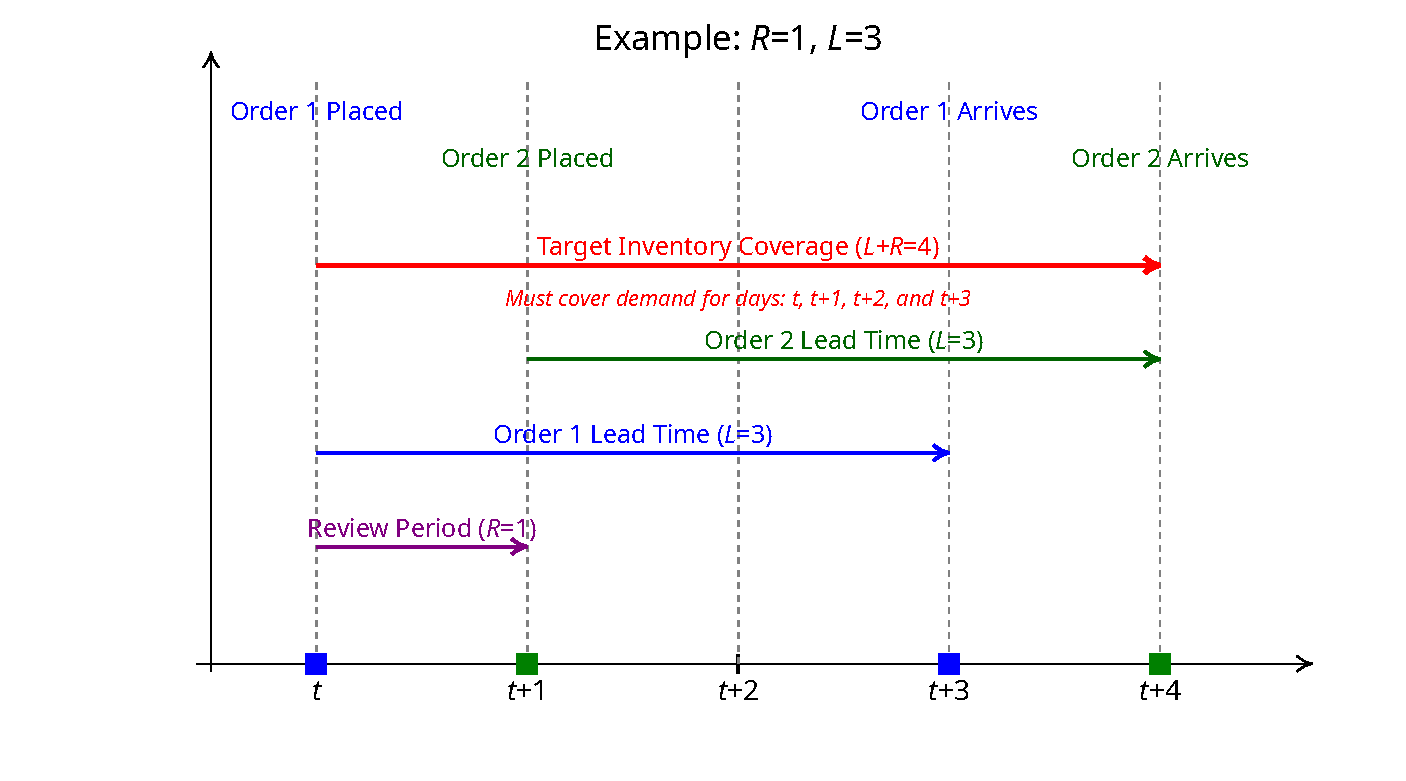
\includegraphics[width=6.5cm]{figures/periodic_replenishment.pdf}
%\caption{Example: $R=1$, $L=4$}
\end{figure}
\end{frame}

\begin{frame}{Distribution of Demand during Exposure Window ($L+R$)}
\begin{small}
The Newsvendor model can be extended to accommodate positive lead times and periodic reviews.
\begin{itemize}
\item \textbf{Key Idea}: Optimize for the total demand during the exposure period ($L+R$), rather than a single period:
$$D_t^{L+R} = D_t + D_{t+1} + \dots + D_{t+L+R-1}$$
\item Assuming independent periods, the probability distribution of $D_t^{L+R}$ is computed by convolving the individual demand distributions.
\item If the lead time ($L$) is stochastic, the distribution of $D_{t}^{L+R}$ becomes a mixture distribution. It weights the cumulative demand ($S_{t, l+R} = D_t + \cdots + D_{t+l+R-1}$) across all possible lead times up to a maximum $\bar{L}$:
\begin{align*}
\mathbb{P}({D}^{L+R}_{t} = k) &= \sum_{l=1}^{\bar{L}} \mathbb{P}(S_{t, l + R}=k)\mathbb{P}(L=l)
\end{align*}
\end{itemize}
\end{small}
\end{frame}

\begin{frame}[plain]
\centering
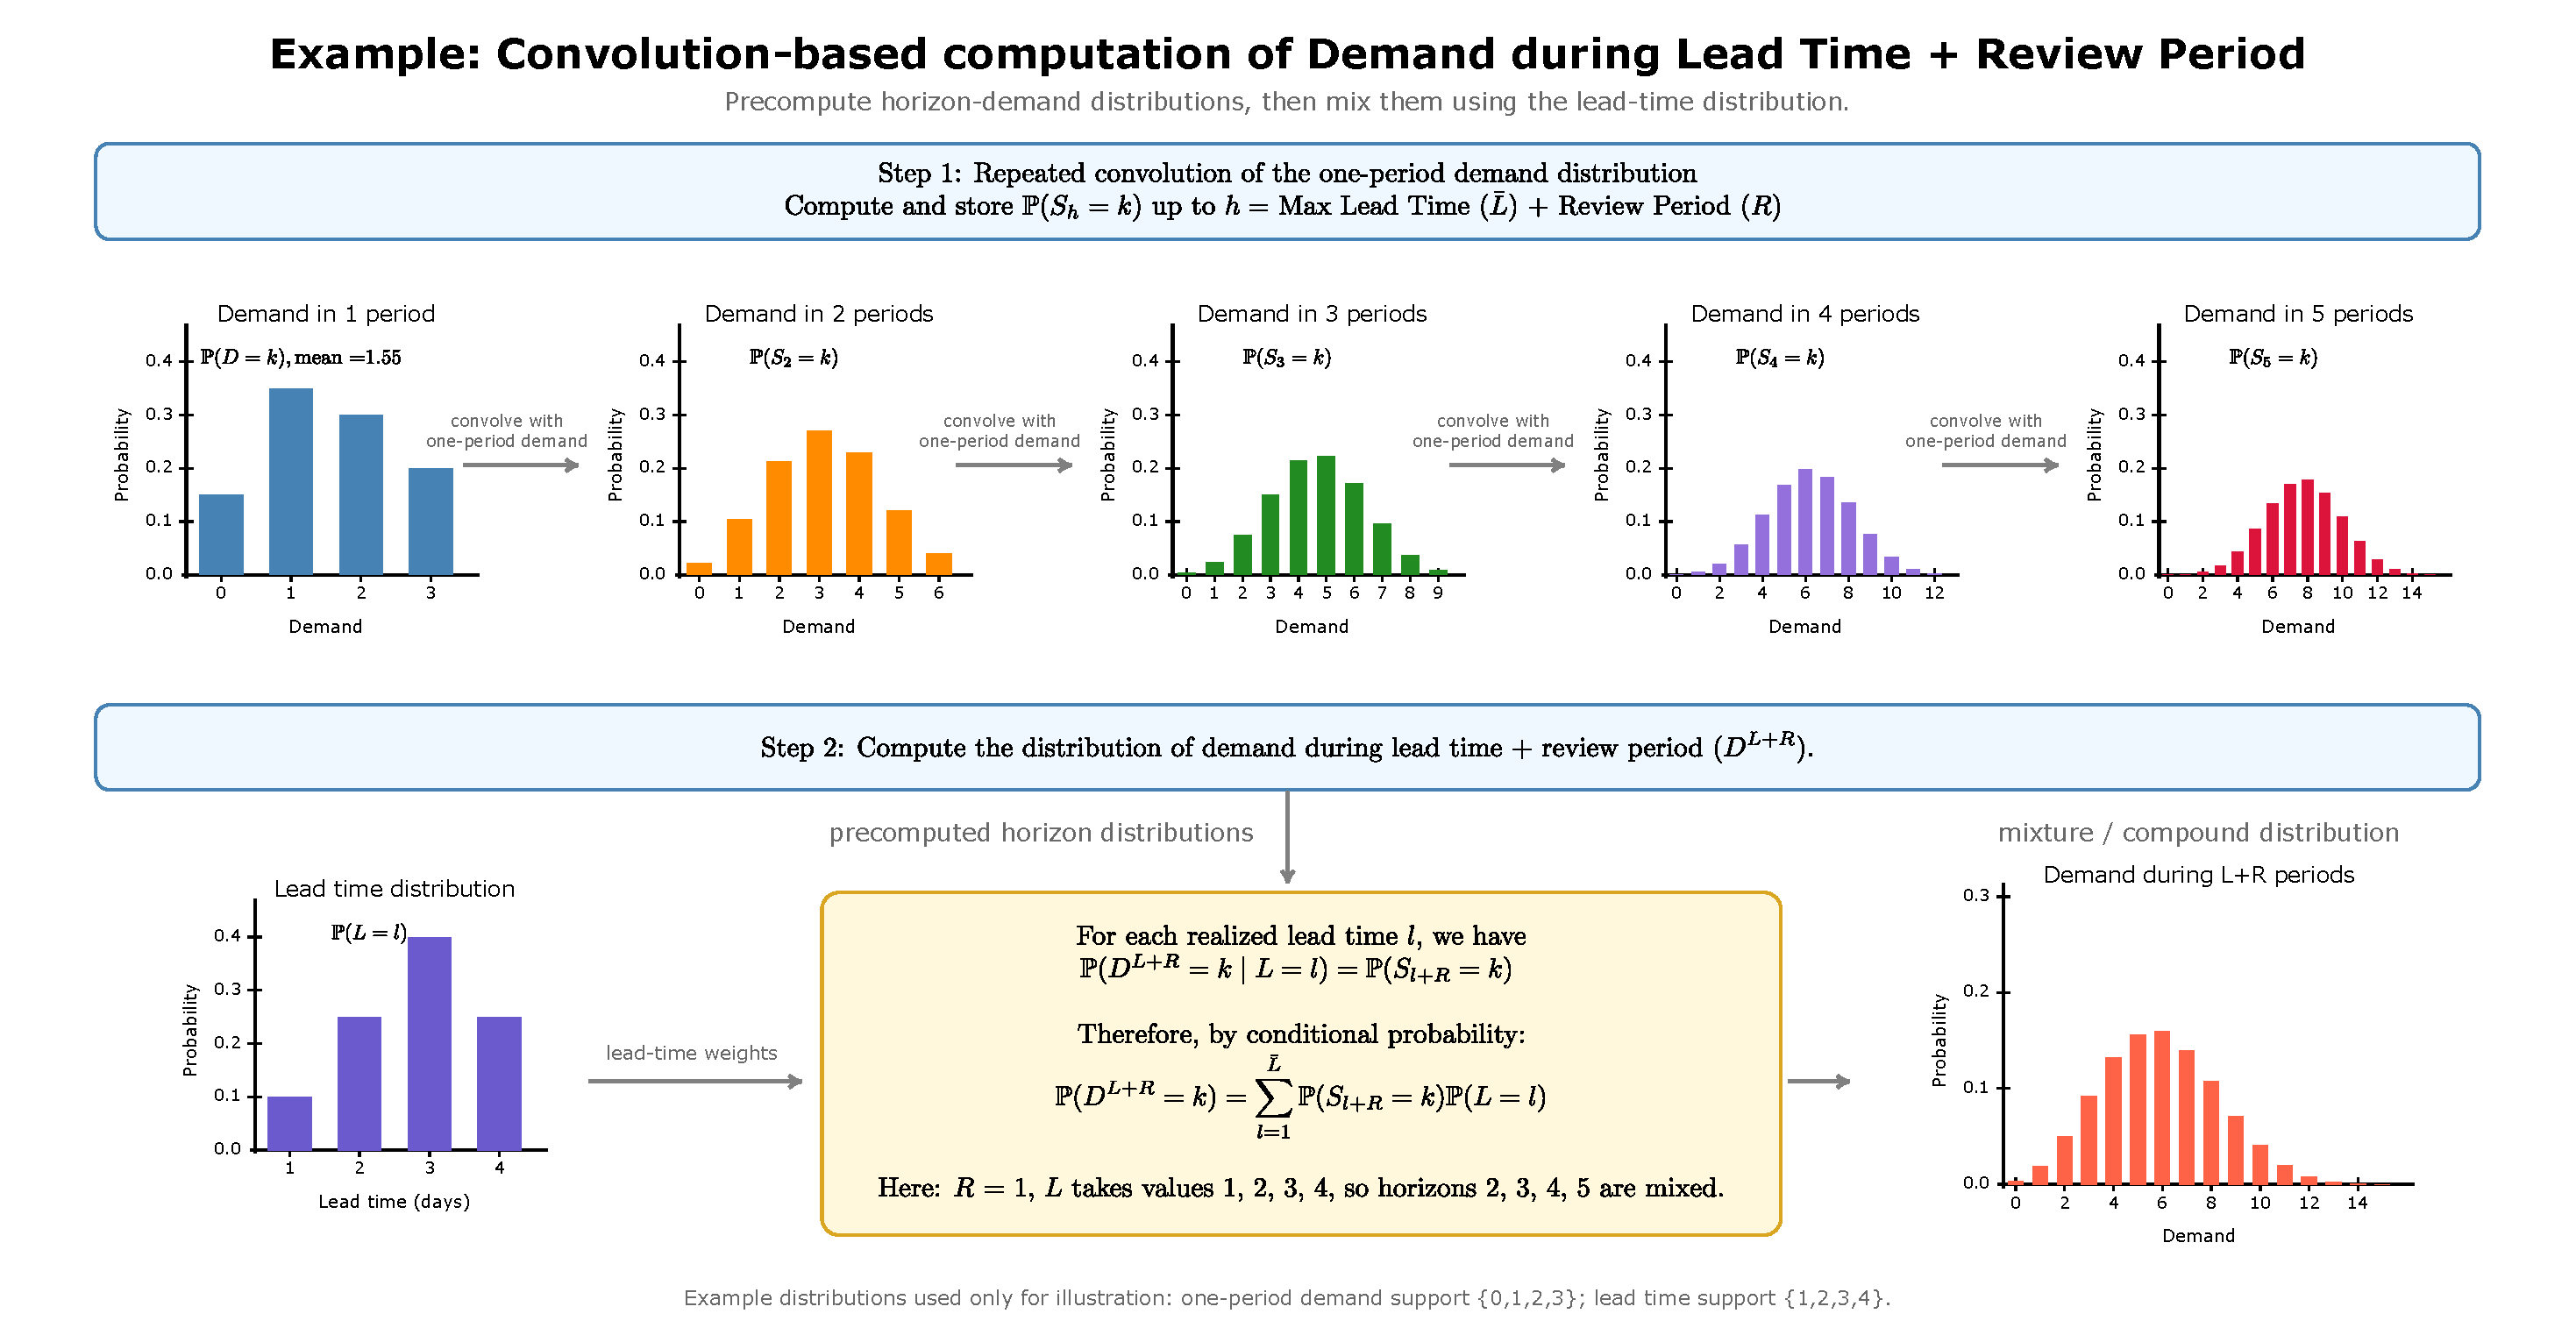
\includegraphics[width=\textwidth,height=\textheight,keepaspectratio]{figures/convolution_leadtime_figure.pdf}
\end{frame}

\section{Stochastic Inventory Optimization}
\begin{frame}{Multi-Product Newsvendor with Budget Constraint}
\begin{itemize}
% \item A decision-maker needs to place orders for $N$ distinct products while satisfying a budget constraint.
\item A decision-maker needs to determine the target inventory for $N$ distinct products while satisfying a working capital constraint\footnote{\textcite{zhang2009} considered a similar formulation. \textcite{perakis2020} further extended this to multi-item, multi-warehouse settings under dual capacity constraints.}.
\item The total capital tied up in the target inventory cannot exceed a predefined working capital limit, denoted as $B$.
%\item The total cost of purchasing all the products cannot exceed a budget limit ($B$).
\item Inputs:
\begin{itemize}
% \item Number of products: $N$
\item Demand during lead time + review period ($D_i$): Random variable with CDF $F_i(\cdot)$ 
\item Economic parameters for product $i$:
\begin{itemize}
\item Selling price of product $i$: $p_i$ per unit
\item Purchase cost of product $i$: $c_i$ per unit
% \item Salvage value of product $i$: $s_i$ per unit. Typically, $p_i > c_i > s_i$.
\item Shortage penalty of product $i$: $r_i$ per unit. 
\end{itemize}
\item Available budget: $B$
\end{itemize}
\end{itemize}
\end{frame}

\begin{frame}{Problem Formulation}
\begin{itemize}
\item The profit from the sales of product $i$, denoted as $P_i(x_i)$, balances revenue against purchase costs and shortage penalties for the target inventory $x_i$:
\begin{equation*}
P_i(x_i) = p_i \min\{D_i, x_i\} - c_i x_i - r_i \max\{D_i-x_i, 0\}
\end{equation*}
\item Goal: Maximize the total expected profit across all $N$ products:
\begin{equation*}
P(x_1, \cdots, x_N) = \sum_{i=1}^N \mathbb{E}[P_i(x_i, D_i)]
\end{equation*}
\item The Constraint: The total working capital required to fund the target inventory must not exceed the available limit $B$:
\begin{equation*}
\sum_{i=1}^N c_i x_i \leq B
\end{equation*}
\end{itemize}
\end{frame}

\begin{frame}[allowframebreaks]{Solving via Binary Search}
\begin{small}
\begin{itemize}
\item We relax the hard working capital constraint by introducing a non-negative Lagrange multiplier, $\lambda \geq 0$. This translates the constrained problem into an unconstrained maximization:
\begin{equation*}
\text{Maximize } \mathcal{L}(x_1, \cdots, x_N, \lambda) = \sum_{i=1}^N \mathbb{E}[P_i(x_i, D_i)] - \lambda \left(\sum_{i=1}^N c_i x_i - B\right)
\end{equation*}
\item This is equivalent to a standard newsvendor problem where the effective cost is adjusted to $c_i' = c_i+\lambda$. The optimal $x_i^*(\lambda)$ is given by:
\begin{equation*}
x_i^*(\lambda) = F_i^{-1}\left( \frac{p_i-c_i (1+\lambda)+r_i}{p_i+r_i} \right)
\end{equation*}
\item Consequently, the total working capital tied up by this optimal solution, $C(\lambda) = \sum_i^N c_i x_i^*(\lambda)$, acts as a non-increasing function of $\lambda$.
\end{itemize}
\end{small}

\framebreak
\begin{small}
\begin{itemize}
\item Our objective is to find the smallest value of $\lambda \geq 0$ such that the total cost $C(\lambda)$ satisfies the working capital constraint $C(\lambda) \leq B$.
\item Because $C(\lambda)$ is monotonic with respect to $\lambda$, we can efficiently locate the optimal $\lambda$ using a binary search.
\item The Procedure:
\begin{itemize}
\item First, check the unconstrained solution ($\lambda=0$). If $C(0) \leq B$, then $x_i^*(0)$ is the optimal order quantity for all products. 
\item If the budget is exceeded, initiate a binary search over the interval $[0, \lambda_{\text{max}}]$, where $\lambda_{\text{max}} = \min_{i=1,\cdots, N}\left(\frac{p_i+r_i}{c_i}-1\right)$.
\item Set $\lambda_L=0$, $\lambda_U = \lambda_{\text{max}}$, and evaluate the midpoint $\lambda_M = (\lambda_U + \lambda_L)/2$.
\item If $C(\lambda_M)>B$, then $\lambda_M$ is too small; continue the search in $[\lambda_M, \lambda_U]$. 
\item If $C(\lambda_M)\leq B$, then $\lambda_M$ is potentially feasible but might be too large; continue the search in $[\lambda_L, \lambda_M]$. 
\end{itemize}
\end{itemize}
\end{small}
\end{frame}

\section{Conclusion}

\begin{frame}{Takeaways}
\begin{itemize}
\item Forecasts are not the objective, inventory decisions are. 
% \item Point forecasts are insufficient when inventory decisions depend on service levels and asymmetric costs.

\item Probabilistic forecasting estimates the entire conditional demand distribution: $\mathbb{P}(D_{t+\tau}\mid x_t)$

\item Lead time and review period uncertainty are propagated by computing the distribution of cumulative demand:
\begin{align*}
D^{L+R}_{t} = D_{t+1} + \cdots + D_{t+L+R}
\end{align*}
\item Inventory targets are obtained by solving a stochastic optimization problem that explicitly accounts for
\begin{itemize}
    \item service level requirements,
    \item holding and shortage costs,
    \item and working capital constraints.
\end{itemize}
\end{itemize}

\end{frame}

\begin{frame}[t,allowframebreaks]{References}
\begin{footnotesize}
\printbibliography
\end{footnotesize}
\end{frame}

\end{document}